\chapter{TINJAUAN PUSTAKA}
\label{chap:tinjauanpustaka}


\section{Hasil penelitian/perancangan terdahulu}
Dalam penelitian ini, penulis merujuk pada beberapa studi sebelumnya yang relevan. Penelitian-penelitian tersebut memiliki hubungan dengan topik yang sedang diteliti, sehingga dapat digunakan sebagai dasar untuk penelitian ini.

\subsection{\emph{Autonomous Thermal Vision Robotic System for Victims Recognition}}

Penelitian oleh Cruz Ulloa mengembangkan robot berkaki empat (\emph{quadruped-legged}) menggunakan \emph{Unitree A1} yang dilengkapi dengan kamera termal \emph{Optris Pi640}. Robot ini dirancang untuk mendeteksi korban dalam misi pencarian dan penyelamatan di lingkungan pasca-bencana, dengan memanfaatkan citra termal yang dianalisis menggunakan algoritma \emph{Convolutional Neural Network (CNN)}. Hasil penelitian menunjukkan bahwa sistem ini mampu mencapai akurasi deteksi lebih dari 90\% dalam kondisi ekstrem, seperti lingkungan minim cahaya atau area yang dipenuhi puing bangunan. Robot ini beroperasi secara \emph{teleoperated} dan mampu menjelajah medan yang tidak rata, sehingga sangat membantu tim pencarian dalam menemukan korban yang terperangkap di lokasi bencana \cite{Cruz2021}. Sistem robot dibangun dengan menggunakan \emph{Robot Operating System (ROS) 1 Melodic}, seperti pada gambar \ref{fig:Quadruped dengan kamera termal untuk deteksi korban}

\begin{figure} [H] \centering
  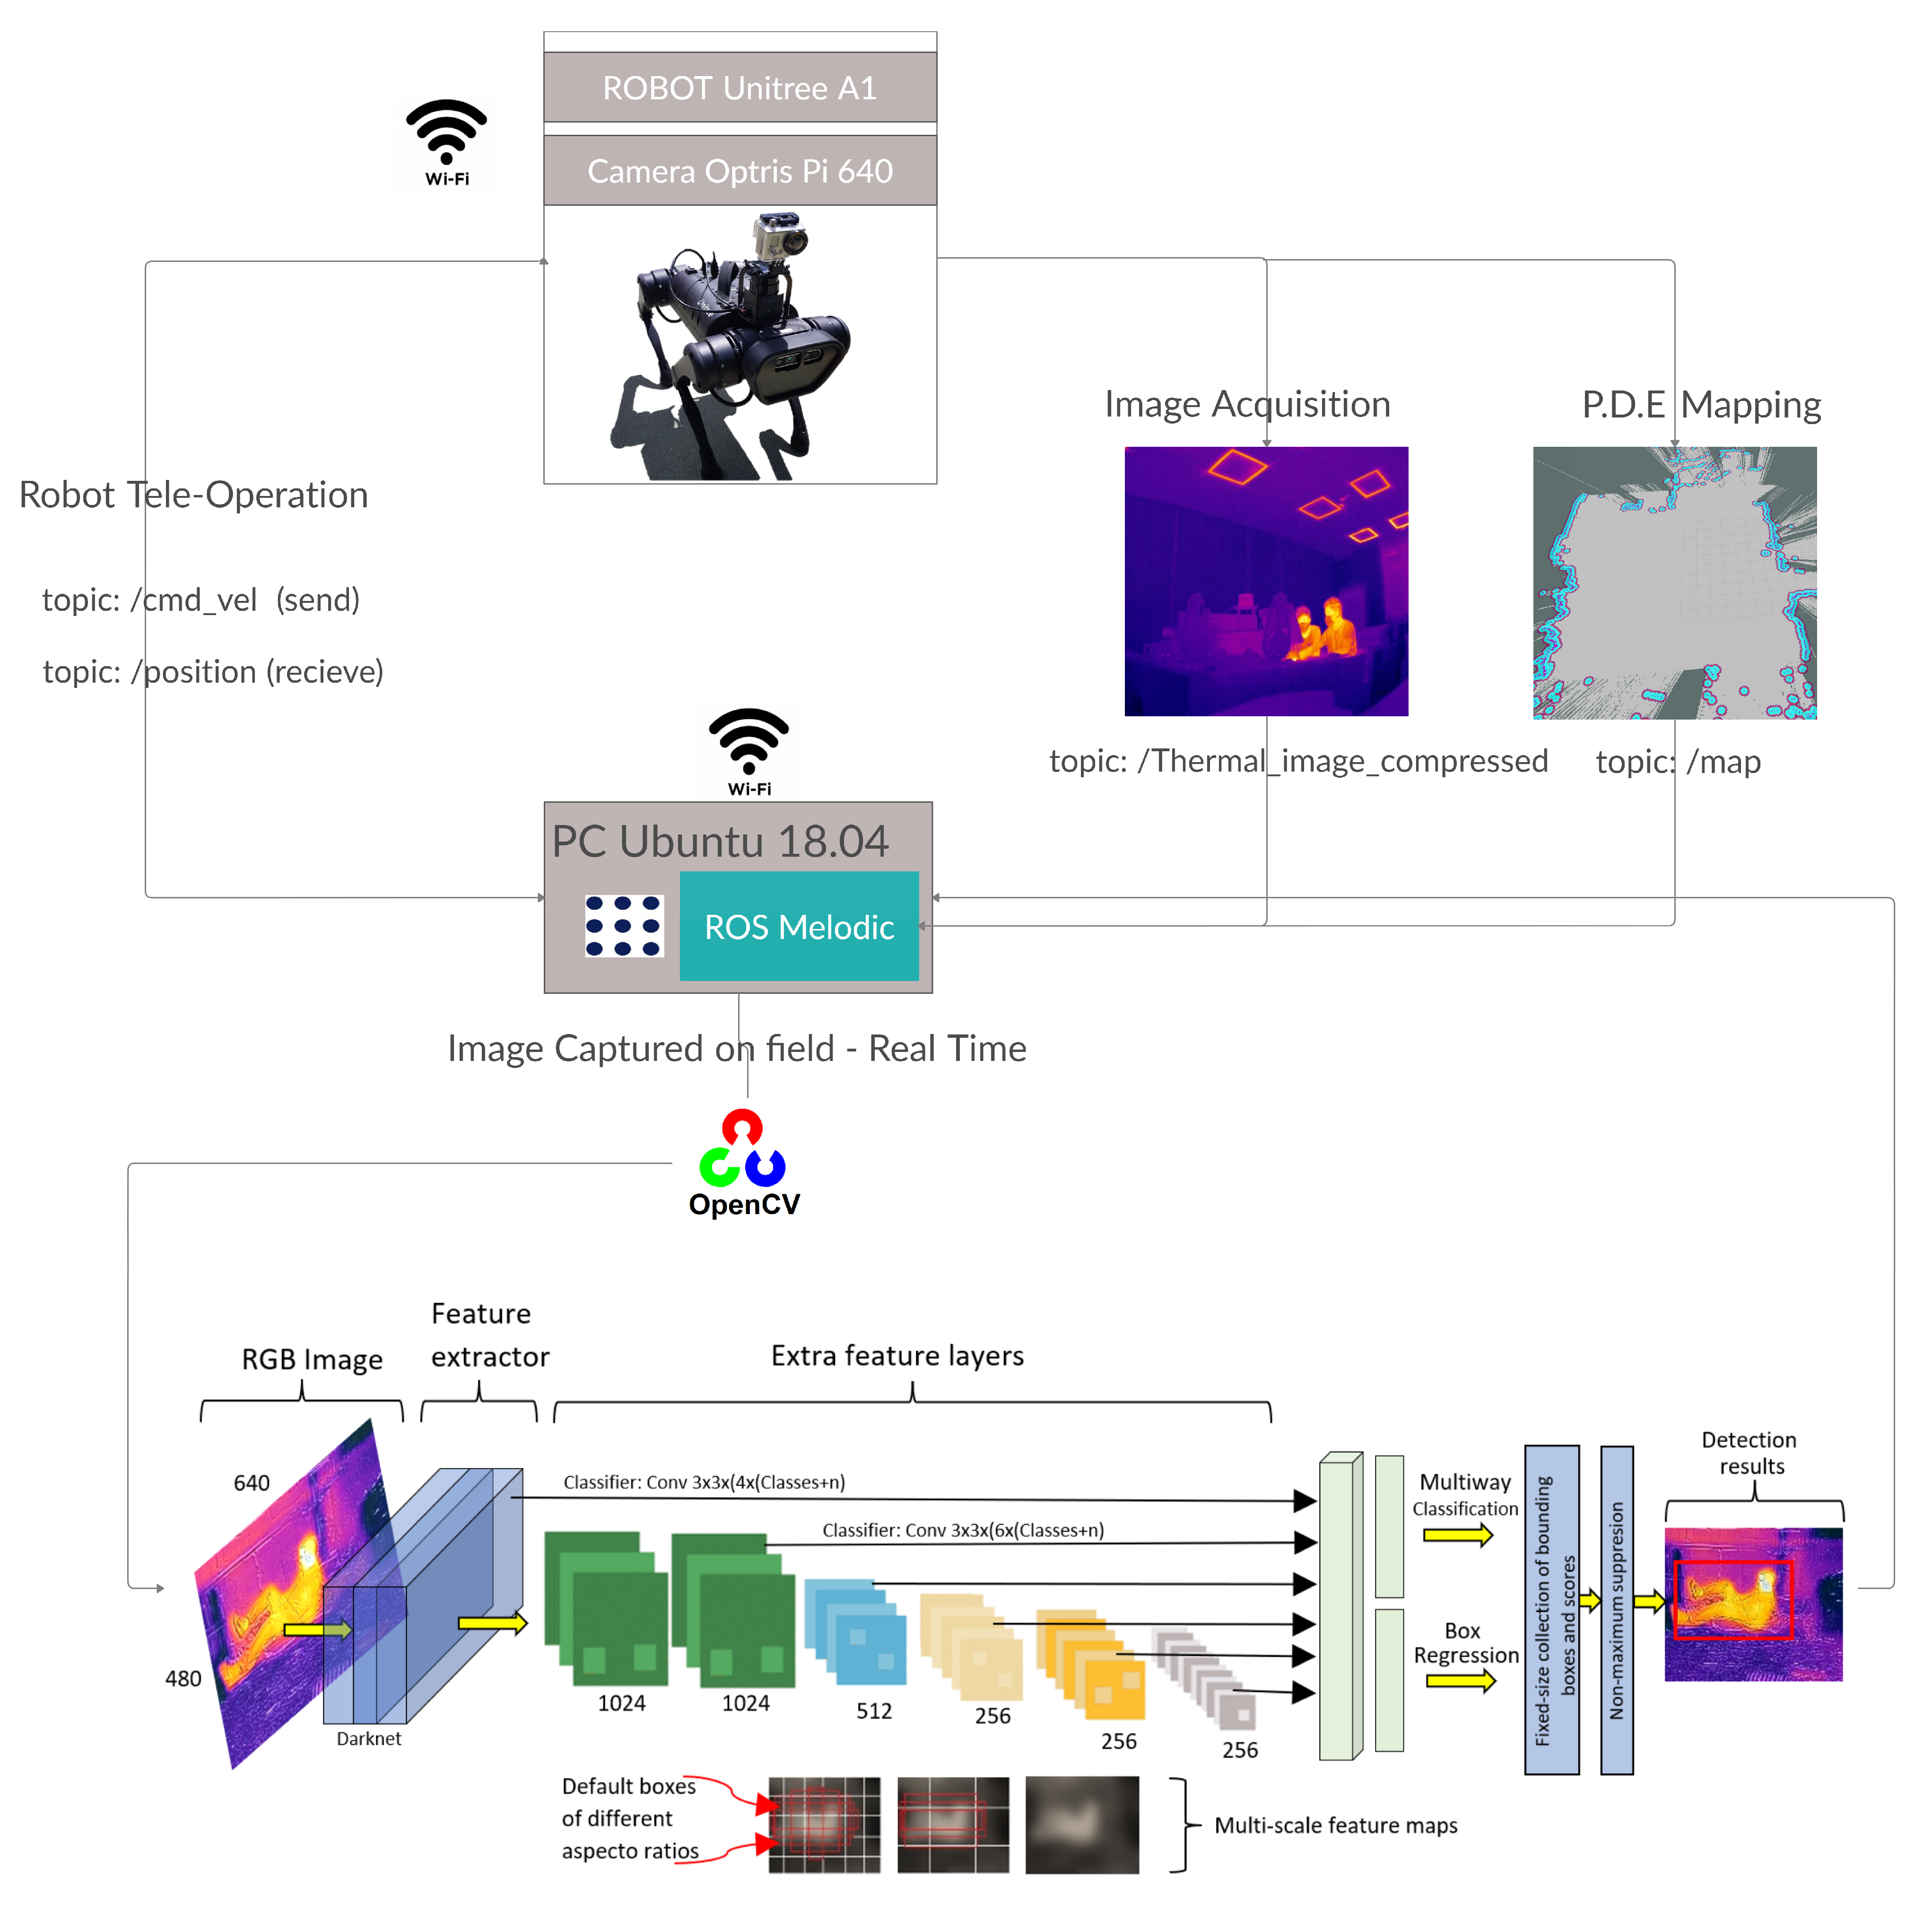
\includegraphics[scale=0.057]{gambar/bab2/unitreea1.png}
  \caption{\emph{Quadruped robot} dengan kamera termal untuk deteksi korban}
  \label{fig:Quadruped  dengan kamera termal untuk deteksi korban}
  \footnotesize{\textbf{Sumber:} Cruz Ulloa (2021)}
\end{figure}

Penelitian ini memiliki kesamaan dengan topik yang sedang dikembangkan, yaitu penggunaan robot \emph{quadruped} dan kamera termal untuk memberikan estimasi posisi objek dalam peta, menjadikannya sangat relevan dengan pendekatan yang sedang dirancang.



\subsection{\emph{Image Processing Technique Applied to Electrical
Substations Based on Drones With Thermal Vision
for Predictive Maintenance}}
Penelitian ini mengusulkan penggunaan \emph{VANT} (Vehículo Aéreo No Tripulado) atau drone, yang dilengkapi dengan dua jenis kamera: \emph{kamera tradisional} untuk menangkap gambar visual dan \emph{kamera termografik} untuk memperoleh gambar inframerah yang dapat menunjukkan suhu komponen di gardu induk. Drone ini dilengkapi dengan sistem navigasi dan pengendalian yang memungkinkan operasi otonom di sekitar gardu induk. Data gambar yang diambil oleh drone diproses menggunakan teknik \emph{image processing} untuk mengidentifikasi \emph{hot spots} atau titik panas pada komponen gardu induk.

\begin{figure} [H] \centering
  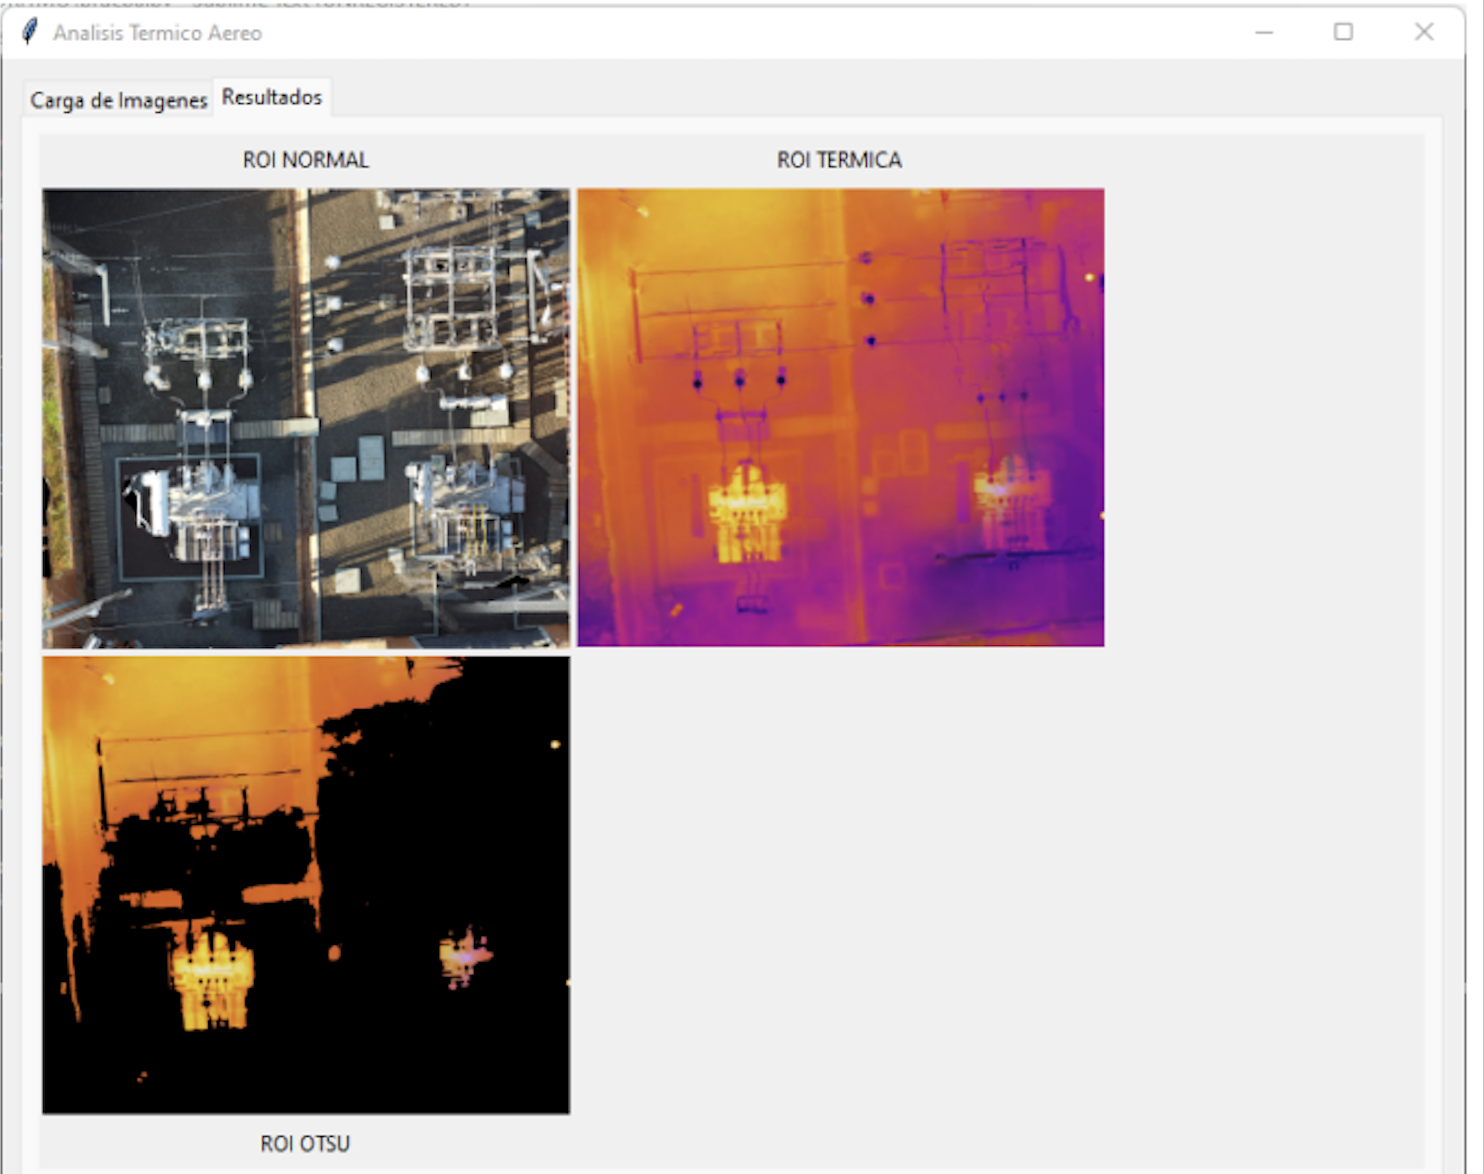
\includegraphics[scale=0.64]{gambar/bab2/drone.png}
  \caption{Drone dengan kamera termal untuk pemantauan gardu induk}
  \label{fig:Drone dengan kamera termal untuk pemantauan gardu induk}
  \footnotesize{\textbf{Sumber:} Prieto et al. (2022)}
\end{figure}

Hasil analisis ini dapat digunakan untuk memprediksi potensi kerusakan pada komponen dan mengambil tindakan pencegahan yang diperlukan. Penelitian ini menunjukkan bahwa penggunaan drone dengan kamera termal dapat meningkatkan efisiensi dan akurasi dalam pemantauan gardu induk, serta meminimalkan risiko keselamatan bagi petugas yang harus melakukan inspeksi langsung di lokasi gardu \cite{Prieto2022}. Penelitian ini memiliki kesamaan dengan topik kami yang juga menggunakan kamera termal untuk pemantauan komponen gardu listrik.

\section{Teori/Konsep Dasar}
Subbab ini membahas berbagai teori dan konsep dasar yang menjadi landasan dalam penyusunan tugas akhir. Penjelasan dalam bab ini mencakup berbagai teori yang relevan dan digunakan dalam pelaksanaan penelitian.

\subsection{Gardu Listrik}
\sloppy
Gardu listrik merupakan salah satu komponen vital dalam sistem kelistrikan yang berfungsi sebagai titik penghubung antara pembangkit listrik dan jaringan distribusi. Melalui gardu listrik, aliran energi listrik dapat diatur dan dialirkan secara efisien dari sumber pembangkit menuju konsumen akhir \cite{stevenson1994power}. Proses transmisi dan distribusi energi listrik tidak dapat dilakukan secara aman dan terkontrol tanpa adanya gardu listrik. Secara umum, terdapat beberapa jenis gardu listrik, antara lain gardu induk dan gardu pembangkit. Gardu induk memiliki fungsi utama untuk menurunkan tegangan listrik dari tingkat tinggi, yang digunakan dalam proses transmisi, menjadi tegangan menengah atau rendah agar aman untuk digunakan oleh konsumen \cite. Gardu ini umumnya terletak di antara pembangkit dan kawasan konsumen, baik permukiman maupun kawasan industri.

Sementara itu, gardu pembangkit merupakan fasilitas yang berada di dekat sumber energi primer, seperti pembangkit listrik tenaga air (PLTA), pembangkit listrik tenaga uap (PLTU), atau jenis pembangkit lainnya. Gardu ini berfungsi untuk menyalurkan energi listrik yang dihasilkan dari proses konversi energi primer ke jaringan transmisi. Untuk mendukung fungsinya, gardu listrik dilengkapi dengan berbagai peralatan kelistrikan, seperti transformator, pemutus sirkuit, dan isolator untuk menjamin keandalan sistem. Keandalan gardu listrik sangat berpengaruh terhadap kualitas dan kontinuitas pasokan energi listrik \cite{gonen2016electric}.

\subsubsection{2.2.1.1 Transformator}
Transformator merupakan salah satu komponen utama dalam gardu listrik yang berfungsi untuk mengubah tingkat tegangan sesuai kebutuhan dalam proses transmisi maupun distribusi energi listrik. Salah satu jenis transformator yang umum pada gardu listrik adalah transformator daya. Transformator daya digunakan untuk menyesuaikan tegangan agar sesuai dengan kebutuhan sistem, sekaligus meminimalkan rugi-rugi daya selama proses transmisi jarak jauh. Berdasarkan fungsinya, transformator daya dibedakan menjadi dua jenis, yaitu transformator \emph{step-up} dan transformator \emph{step-down}  Transformator \emph{step-up} digunakan di sisi pembangkit untuk menaikkan tegangan listrik ke tingkat yang lebih tinggi agar transmisi lebih efisien dan rugi daya berkurang, sedangkan transformator \emph{step-down} digunakan di sisi distribusi untuk menurunkan tegangan ke tingkat yang lebih rendah sehingga aman digunakan oleh konsumen . Transformator daya biasanya dirancang untuk beroperasi pada suhu maksimum sekitar 105\textdegree{}C hingga 110\textdegree{}C, tergantung pada kelas isolasi termal yang digunakan, seperti kelas A, B, atau F \cite{stevenson1994power}.

\subsubsection{2.2.1.2 \emph{Arrester}}
\emph{Arrester}, atau \emph{lightning arrester}, merupakan perangkat pelindung dalam sistem kelistrikan yang berfungsi untuk mengamankan peralatan dari lonjakan tegangan akibat sambaran petir atau gangguan tegangan lebih sesaat. \emph{Arrester} bekerja dengan cara mengalihkan arus lebih tersebut langsung ke \emph{ground}, sehingga mencegah terjadinya kerusakan pada peralatan penting seperti transformator, pemutus sirkuit, dan komponen lainnya di gardu listrik. Pemeliharaan rutin terhadap \emph{arrester} sangat penting dilakukan untuk memastikan performanya tetap optimal. Salah satu parameter penting yang harus dipantau adalah suhu operasi perangkat. Umumnya, \emph{arrester} dirancang untuk beroperasi pada suhu lingkungan antara -40\textdegree{}C hingga 60\textdegree{}C. Jika suhu operasional melebihi batas maksimum tersebut, maka dapat terjadi kerusakan permanen pada komponen internal arrester yang berakibat pada menurunnya efektivitas perlindungan sistem secara keseluruhan \cite{Kartika2022}.

\subsubsection{2.2.1.3 Disconnector}
\emph{Disconnector} merupakan perangkat yang berfungsi untuk memisahkan suatu bagian dari sistem kelistrikan guna keperluan pemeliharaan atau perbaikan, tanpa memengaruhi bagian lain dari jaringan. Pemeliharaan serta pengujian secara berkala terhadap \emph{disconnector} sangat krusial untuk memastikan bahwa perangkat ini dapat berfungsi secara optimal saat dibutuhkan. Suhu operasi \emph{disconnector} umumnya berada dalam kisaran 20°C hingga 40°C. Namun, apabila suhu meningkat melebihi 85°C, dapat terjadi overheating yang berpotensi menyebabkan kegagalan fungsi \cite{Henriana2022}.


\subsubsection{2.2.1.4 Busbar}
\emph{Busbar} adalah komponen dalam gardu listrik yang berfungsi sebagai penghubung antara berbagai peralatan listrik. \emph{Busbar} memungkinkan distribusi arus listrik yang efisien dan aman di dalam gardu. \emph{Busbar} biasanya terbuat dari bahan konduktif yang baik, seperti tembaga atau aluminium, dan dirancang untuk menampung arus listrik dalam jumlah besar. Pemeliharaan dan pengujian \emph{busbar} secara rutin diperlukan untuk mencegah kerusakan dan memastikan keandalan sistem distribusi listrik. Suhu operasi \emph{busbar} dapat bervariasi, tetapi umumnya tidak boleh melebihi 90°C untuk mencegah overheating yang dapat merusak isolasi dan struktur busbar itu sendiri \cite{Telaumbanua2024}.

\subsubsection{2.2.1.5 Isolator}
\emph{Isolator} adalah perangkat yang berfungsi untuk memisahkan bagian dari sistem kelistrikan, sehingga mencegah arus listrik mengalir ke bagian yang tidak diinginkan. \emph{Isolator} digunakan untuk menjaga keamanan dan keandalan sistem kelistrikan, terutama saat pemeliharaan dilakukan. \emph{Isolator} dirancang untuk menahan tegangan tinggi dan memiliki karakteristik dielektrik yang baik. Pemeliharaan \emph{isolator} juga penting untuk memastikan bahwa tidak ada kebocoran arus yang dapat menyebabkan kerusakan pada peralatan lainnya. Suhu operasi \emph{isolator} biasanya berkisar antara -30°C hingga 50°C, dan overheating dapat terjadi jika suhu melebihi 70°C, yang dapat mengakibatkan kerusakan pada material isolasi \cite{Moreno2017}.

\subsubsection{2.2.1.6 Pemutus Sirkuit (\emph{Circuit Breaker})}
\emph{Pemutus sirkuit} adalah perangkat yang berfungsi untuk melindungi sistem kelistrikan dari arus lebih (\emph{overcurrent}) dan hubung singkat (\emph{short circuit}). \emph{Pemutus sirkuit} dapat secara otomatis memutuskan aliran listrik ketika terdeteksi adanya gangguan, sehingga mencegah kerusakan pada peralatan dan menjaga keselamatan sistem. Terdapat berbagai jenis \emph{pemutus sirkuit}, termasuk \emph{pemutus sirkuit otomatis} (\emph{automatic circuit breaker}) dan \emph{pemutus sirkuit manual} (\emph{manual circuit breaker}), yang masing-masing memiliki aplikasi dan karakteristik yang berbeda Pemeliharaan dan pengujian berkala terhadap \emph{pemutus sirkuit} sangat penting untuk memastikan bahwa perangkat ini berfungsi dengan baik saat dibutuhkan. Suhu operasi \emph{pemutus sirkuit} biasanya berkisar antara -25°C hingga 55°C, dan overheating dapat terjadi jika suhu melebihi 85°C, yang dapat menyebabkan kerusakan pada mekanisme pemutus \cite{Ilomets2020}.

\subsection{DeepRobotics Jueying X30 Pro}
\textit{DeepRobotics Jueying X30 Pro} adalah robot berkaki empat (\textit{quadruped}) generasi terbaru yang dikembangkan oleh perusahaan teknologi robotik DeepRobotics di Tiongkok. Dirancang untuk berbagai aplikasi industri seperti inspeksi fasilitas, penyelamatan darurat, eksplorasi lingkungan ekstrem, serta pemantauan di berbagai medan, robot ini mengintegrasikan teknologi sensor canggih untuk navigasi dan persepsi lingkungan. Dalam memdukung navigasi dan pemetaan lingkungan, X30 Pro dilengkapi dengan empat sensor LiDAR 360° Livox dua di bagian depan dan dua di bagian belakang.  Selain itu, X30 Pro dilengkapi dengan IMU (\textit{Inertial Measurement Unit}) Yesense YIS100-V, yang menggabungkan akselerometer dan giroskop untuk mengukur percepatan linear dan kecepatan sudut. 
Dengan desain industrial yang tangguh, \textit{Jueying X30 Pro} mampu bergerak secara cepat dan stabil di berbagai jenis permukaan. Kemampuan tersebut didukung oleh integrasi teknologi persepsi multimodal dan sistem kendali gerak adaptif, sehingga memungkinkan navigasi otonom dalam kondisi lingkungan yang kompleks. Spesifikasi teknis utama dari \textit{X30 Pro} ditampilkan pada Tabel~\ref{tab:spesifikasiX30}.


\begin{table}[H]
	\centering
	\caption{Spesifikasi Teknis Deep Robotics X30}
	\label{tab:spesifikasiX30}
	\renewcommand{\arraystretch}{1.2}
	\begin{tabular}{|p{5.5cm}|p{7cm}|}
		\hline
		\textbf{Parameter}            & \textbf{Spesifikasi}                                              \\
		\hline
		Dimensi (P × L × T)           & 1000 mm × 585 mm × 470 mm                                         \\
		\hline
		Bobot (berat bersih)          & 56--59 kg                                                         \\
		\hline
		Kecepatan Maksimal            & 4 m/s                                                             \\
		\hline
		Kemampuan Menanjak            & Hingga 45\textdegree{} (termasuk tangga terbuka)                  \\
		\hline
		Ketinggian Rintangan Maksimal & $\geq$ 20 cm                                                      \\
		\hline
		Rentang Suhu Operasional      & --20\textdegree{}C hingga +55\textdegree{}C                       \\
		\hline
		Perlindungan Lingkungan       & IP67 (tahan air dan debu)                                         \\
		\hline
		Daya Tahan Baterai            & 2,5--4 jam (dengan beban penuh)                                   \\
		\hline
		Sistem Pengisian Daya         & Pengisian otomatis (\emph{auto-charging}), \emph{manual charging} \\
		\hline
		Antarmuka Komunikasi          & Ethernet, USB 2.0/3.0, dan Wi-Fi                                  \\
		\hline
	\end{tabular}
	\footnotesize\\ \textbf{Sumber:} DEEP Robotics (2023)
\end{table}


\noindent
Untuk mendukung operasi otonom dan efisien, \emph{DeepRobotics Jueying X30 Pro} dilengkapi dengan tiga unit komputer onboard yang masing-masing bertanggung jawab atas fungsi gerak (\emph{motion}), persepsi (\emph{perception}), dan navigasi (\emph{navigation}). Arsitektur ini memungkinkan pemrosesan paralel dan spesialisasi tugas, meningkatkan kinerja robot dalam lingkungan yang kompleks dan dinamis. Ketiga komputer ini terhubung melalui  Ethernet seperti pada gambar \ref{fig:network_architecture_x30pro}
\begin{figure}[H]
  \centering
  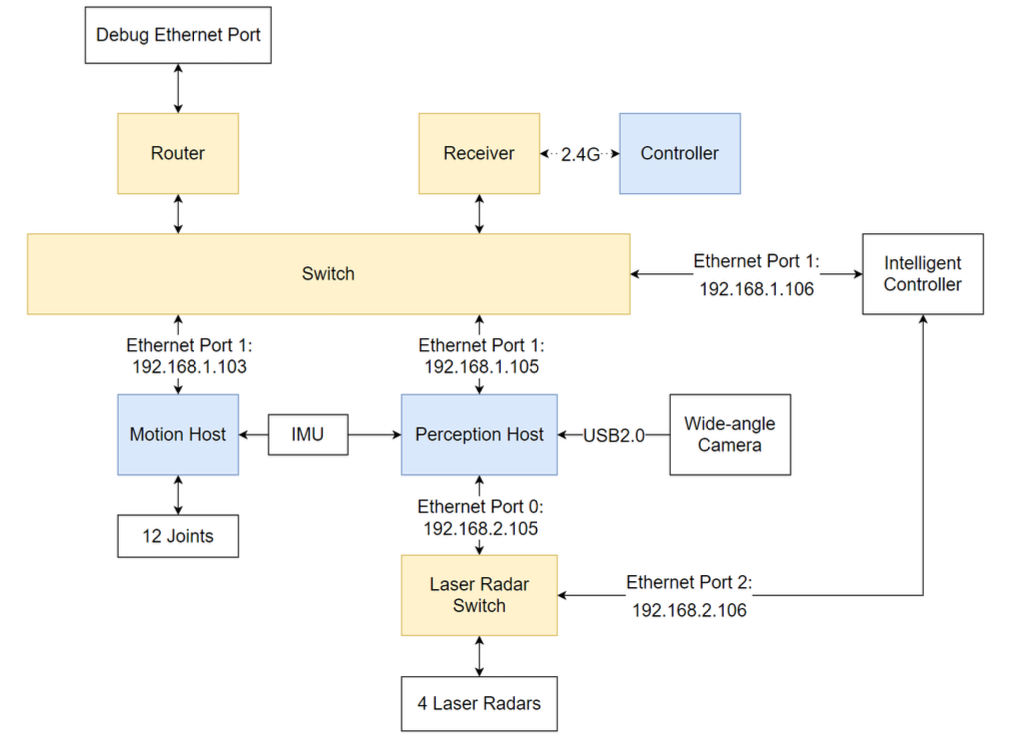
\includegraphics[width=0.75\textwidth]{gambar/bab2/network-x30.png}
  \caption{Arsitektur Jaringan Internal \emph{DeepRobotics Jueying X30 Pro}}
  \label{fig:network_architecture_x30pro}
  \footnotesize{\textbf{Sumber:} DeepRobotics (2023)}
\end{figure}


Arsitektur tersebut memungkinkan pertukaran data yang cepat dan sinkronisasi antar sistem. Arsitektur modular ini tidak hanya meningkatkan efisiensi operasional tetapi juga memudahkan integrasi dengan sistem eksternal dan pembaruan perangkat lunak.



